\chapter{Adicionando elementos a GUI do PD}

\example{
\begin{itemize}
\item \texttt{exitbt-plugin.tcl}
\item \texttt{tripleclick-plugin.tcl}
\item \texttt{canvas-plugin.tcl}
\end{itemize}
}

Uma das finalidades dos pluguins de GUI é adicionar novas funcionalidades ao
PD por meio de sua interface gráfica.
Isto, muitas vezes, significa criar novos Menus, barra de ferramentas, barra
de status e outros elementos gráficos que possam disparar a nova funcionalidade.
Neste capítulo apresentaremos alguns destes elementos.


% -----+-----+-----+-----+-----+-----+-----+-----+-----+-----+-----+-----+-----+
%      |     |     |     |     |     |     |     |     |     |     |     |     |
% -----+-----+-----+-----+-----+-----+-----+-----+-----+-----+-----+-----+-----+
\section{Adicionando Menus}

Criar menu TCL com as opções de nomes de todo mundo.

% -----+-----+-----+-----+-----+-----+-----+-----+-----+-----+-----+-----+-----+
%      |     |     |     |     |     |     |     |     |     |     |     |     |
% -----+-----+-----+-----+-----+-----+-----+-----+-----+-----+-----+-----+-----+
\section{Adicionando Ações ao Menu pop-up}


% -----+-----+-----+-----+-----+-----+-----+-----+-----+-----+-----+-----+-----+
%      |     |     |     |     |     |     |     |     |     |     |     |     |
% -----+-----+-----+-----+-----+-----+-----+-----+-----+-----+-----+-----+-----+
\section{Adicionando elementos ao canvas}

Status bar com canvas name

Ver as variáveis globais
Ver as funções principais
Ver as classes e como usá-las

Adicionando elementos e funcionalidades

Desenhando no canvas

Alterando funções existentes


% -----+-----+-----+-----+-----+-----+-----+-----+-----+-----+-----+-----+-----+
%      |     |     |     |     |     |     |     |     |     |     |     |     |
% -----+-----+-----+-----+-----+-----+-----+-----+-----+-----+-----+-----+-----+
\section{Enviando mensagens}

Uma maneira de enviar mensagens do Tcl/tk para o engine do Pd é por meio da
função \courier{::pd\_connect::pdsend}.
Esta função, conforme exemplo do Código \ref{code:sendmessage}, permite enviar
mensagens ao Pure Data.

\begin{lstlisting}[caption={Enviando mensagem para o PD (\courier{tripleclick-plugin.tcl})},
label={code:sendmessage}]
::pd_connect::pdsend "$mytoplevel obj"
\end{lstlisting}


% \url{http://puredata.info/docs/guiplugins/GuiPluginsAPI/}
% https://svn.code.sf.net/p/pure-data/svn/branches/pd-gui-rewrite/0.43/startup/



% -----+-----+-----+-----+-----+-----+-----+-----+-----+-----+-----+-----+-----+
%      |     |     |     |     |     |     |     |     |     |     |     |     |
% -----+-----+-----+-----+-----+-----+-----+-----+-----+-----+-----+-----+-----+
\section{Adicionando novos menus}

Entre as alterções possíveis, está adicionar novos itens a um menu existente.
O Código \ref{code:menu} apresenta algumas possibilidades de comandos para 
adicionar novos menus e itens de menu ao menu principal do Pure Data.

\begin{lstlisting}[caption={Alterando o menu.},label={code:menu}]
.menubar.edit add command -label blob -command { puts teste } -accel

bind all <$::modifier-Shift-Key-Z> {menu_redo}

.menubar add  separator

menu .menubar.align

.menubar add cascade -label Align -menu .menubar.align

.menubar.align add command -label Left -command {puts Left}

.menubar insert 3 cascade -label Align -menu .menubar.align

.menubar.edit insert 3 command -label  test  -command {puts x} -state disabled

bind <<Loaded>> {menubar.edit entryconfigure test -state enabled}
\end{lstlisting}

% -----+-----+-----+-----+-----+-----+-----+-----+-----+-----+-----+-----+-----+
%      |     |     |     |     |     |     |     |     |     |     |     |     |
% -----+-----+-----+-----+-----+-----+-----+-----+-----+-----+-----+-----+-----+
\section{Desenhando no canvas}

A tela para a criação de \patches do Pure Data é um objeto \texttt{canvas} do
TCL.
Neste objeto TCL podemos desenhar diversos componentes gráficos.
Imaginando que a janela do nosso \patch tenha o nome ``.x12be7d0'', o
Código~\ref{code:canvas} apresenta comandos para desenhar no canvas desta
janela.

\begin{lstlisting}[caption={Desenhando componentes gráficos no canvas},label={code:canvas}]
.x12be7d0.c create rectangle 10 10 20 20 -tags my_rectangle

.x12be7d0.c create text 400 200 -text Hello

.x12be7d0.c create oval 100 100 30 50

.x12be7d0.c create polygon 0 0 30 100 50 20 100 50 10 34

.x12be7d0.c create arc 0 0 100 200

.x12be7d0.c create line 0 0 10 10 12 5 15 3 20 12

.x12be7d0.c create image 100 100 -image [image create photo -file /home/flavio/Pictures/csound.gif] -anchor nw
\end{lstlisting}

O resultado destes comandos é apresentado na Fig.\ref{fig:canvas_draw}.

\grafico{canvas_draw}{Desenhando no canvas}


One thing that is tricky to understand is the difference between a Tk
'canvas' and a 'canvas' in terms of Pd's implementation.  They are similar,
but not the same thing.  In Pd code, a 'canvas' is basically a patch, while
the Tk 'canvas' is the backdrop for drawing everything that is in a patch.
The Tk 'canvas' is contained in a 'toplevel' window. That window has a Tk
class of 'PatchWindow'.


Além de desenhar objetos gráficos é possível adicionar widgets TCL ao canvas
do Pure data.
Apesar de ter mencionado que não é objetivo deste material ensinar TCL,
apresentaremos nesta seção vários widgets TCL.
Nesta seção apresentaremos vários exemplos\footnote{Exemplos adaptados do site: \url{http://pages.cpsc.ucalgary.ca/~saul/personal/archives/Tcl-Tk_stuff/tcl_examples/}}
de widgets que podem ser adicinados ao canvas do Pure Data.

Consulte\footnote{\url{http://wiki.tcl.tk/490}} para obter mais informações
sobre ow widgets do TCL.

Para que os exemplos aqui apresentados funcione em seu Pure Data diretamente
a partir do console TCL, o código \ref{code:windowname} deve ser executado
antes de rodar os exemplos.

\begin{lstlisting}[caption={Código para pegar o nome da última janela aberta},
label={code:windowname}]
foreach c [winfo children .] {}
set mylastwindow .[winfo name [lindex $c] ]
\end{lstlisting}

% ------------------------------------------------------------------------------
\section{Label}

Label é o nome de um rótulo de texto utilizado em formulários.

\begin{lstlisting}
label ${mylastwindow}.l1 -text "This is what the default label looks like"
label ${mylastwindow}.l2 -text "This is a yellow label on a blue background" \
    -foreground Yellow \
    -background Blue
label ${mylastwindow}.l3 -text "This is a label in Times 24 font" \
    -font {-family times -size 24}\
    -bg white

${mylastwindow}.c create window 10 20 -window ${mylastwindow}.l1
${mylastwindow}.c create window 10 60 -window ${mylastwindow}.l2
${mylastwindow}.c create window 10 100 -window ${mylastwindow}.l3
\end{lstlisting}


\grafico{label}{Exemplo de Label aplicado ao Canvas}

Removendo estes widgets

\begin{lstlisting}
destroy ${mylastwindow}.l1 ${mylastwindow}.l2 ${mylastwindow}.l3
\end{lstlisting}

% ------------------------------------------------------------------------------
\section{Button}

\begin{lstlisting}
proc doIt {widget} {
    global text
    if {$::dsp == 0} {
        set text "DSP ON"
        pdsend "pd dsp 1"
    } else {
        set text "DSP OFF"
        pdsend "pd dsp 0"
    }
    $widget configure -text $text
}

button ${mylastwindow}.b1 -text "Hello" \
        -command {[list puts $::dsp] "doIt ${mylastwindow}.b1"}

${mylastwindow}.c create window 10 100 -window ${mylastwindow}.b1
\end{lstlisting}

Atenção! Veja o que acontece quando se pressiona o botão Quit!

url{http://www.tcl.tk/man/tcl8.4/TkCmd/button.htm}
\grafico{button}{Exemplo de botão adicionado ao canvas.}

\begin{lstlisting}
destroy ${mylastwindow}.b1 ${mylastwindow}.b2
\end{lstlisting}


% ------------------------------------------------------------------------------
\section{Checkbuttons e RadioButtons}

\begin{lstlisting}
set font helvetica

proc applyIt { } {
    global bold italics font
    if {$bold} {set weight bold} {set weight normal}
    if {$italics} {set slant italic} {set slant roman}
    ${mylastwindow}.c.b configure -font "-family $font -weight $weight -slant $slant"
}

checkbutton ${mylastwindow}.c.c1 -text Bold -variable bold   -anchor w
checkbutton ${mylastwindow}.c.c2 -text Italics -variable italics  -anchor w

radiobutton ${mylastwindow}.c.r1 -text Helvetica -variable font -value helvetica
radiobutton ${mylastwindow}.c.r2 -text Courier   -variable font -value courier   

button ${mylastwindow}.c.b -text Apply \
    -command "applyIt"

applyIt

${mylastwindow}.c create window 10 100 -window ${mylastwindow}.c.c1
${mylastwindow}.c create window 110 100 -window ${mylastwindow}.c.c2
${mylastwindow}.c create window 10 150 -window ${mylastwindow}.c.r1
${mylastwindow}.c create window 110 150 -window ${mylastwindow}.c.r2
${mylastwindow}.c create window 10 200 -window ${mylastwindow}.c.b
\end{lstlisting}

\grafico{check}{Exemplo de radio button e check button.}

\begin{lstlisting}
set font helvetica

proc applyIt { } {
    global bold italics font
    if {$bold} {set weight bold} {set weight normal}
    if {$italics} {set slant italic} {set slant roman}
    ${mylastwindow}.c.b configure -font "-family $font -weight $weight -slant $slant"
}

checkbutton ${mylastwindow}.c.c1 -text Bold -variable bold   -anchor w
checkbutton ${mylastwindow}.c.c2 -text Italics -variable italics  -anchor w

radiobutton ${mylastwindow}.c.r1 -text Helvetica -variable font -value helvetica
radiobutton ${mylastwindow}.c.r2 -text Courier   -variable font -value courier   

button ${mylastwindow}.c.b -text Apply \
    -command "applyIt"

applyIt

destroy ${mylastwindow}.c.c1 ${mylastwindow}.c.c2 ${mylastwindow}.c.r1 ${mylastwindow}.c.r2 ${mylastwindow}.c.b
\end{lstlisting}

% ------------------------------------------------------------------------------
\section{Entry}

\begin{lstlisting}
entry ${mylastwindow}.c.es -width 20 -textvar S(out)
${mylastwindow}.c create window 40 30 -window ${mylastwindow}.c.es
\end{lstlisting}

\grafico{entry}{Entrada de texto}

\begin{lstlisting}
destroy ${mylastwindow}.c.es
\end{lstlisting}

% ------------------------------------------------------------------------------
\section{Scale}

\begin{lstlisting}
scale ${mylastwindow}.c.s01 -from 100 -to 0 -label "x" -command {puts }

${mylastwindow}.c create window 20 20 -window ${mylastwindow}.c.s01
\end{lstlisting}

Interessante o fato de o parâmetro ser passado automaticamente para o comando
selecionado.

\grafico{scale}{Entrada de texto}

\begin{lstlisting}
destroy ${mylastwindow}.c.s01
\end{lstlisting}

% ------------------------------------------------------------------------------
\section{Spinbox}

\begin{lstlisting}
spinbox ${mylastwindow}.c.sp -from 0.00 -to 5.00 -increment 0.25 -format %5.2f -width 10 \
    -font 10 -justify center -textvariable var -command {::pdwindow::post  "This message will self destruct in five seconds.\n"}
${mylastwindow}.c create window 20 20 -window ${mylastwindow}.c.sp
\end{lstlisting}

\grafico{spin}{Spin}

\begin{lstlisting}
destroy ${mylastwindow}.c.sp
\end{lstlisting}

% ------------------------------------------------------------------------------
\subsection{Text}

\begin{lstlisting}
text ${mylastwindow}.c.t -yscrollcommand "${mylastwindow}.c.t.scroll set" -setgrid true \
        -width 40 -height 10 -wrap word
scrollbar ${mylastwindow}.c.t.scroll -command "${mylastwindow}.c.t yview"
${mylastwindow}.c create window 100 20 -window ${mylastwindow}.c.t
\end{lstlisting}

\url{http://www.tcl.tk/man/tcl8.4/TkCmd/text.htm}

\begin{lstlisting}
destroy ${mylastwindow}.c.t ${mylastwindow}.c.t.scroll
\end{lstlisting}

% ------------------------------------------------------------------------------
\subsection{Listbox}

\begin{lstlisting}
listbox ${mylastwindow}.c.listbox -yscroll "${mylastwindow}.c.listbox.s set"
scrollbar ${mylastwindow}.c.listbox.s -command "${mylastwindow}.c.listbox yview"

${mylastwindow}.c.listbox insert 0 sample stuff colors red yellow green

bind ${mylastwindow}.c.listbox <Double-B1-ButtonRelease> {::pdwindow::post [${mylastwindow}.c.listbox get active]}


${mylastwindow}.c create window 100 100 -window ${mylastwindow}.c.listbox
\end{lstlisting}

\grafico{listbox}{Listbox}

\begin{lstlisting}
destroy ${mylastwindow}.c.listbox ${mylastwindow}.c.listbox.s
\end{lstlisting}

% ------------------------------------------------------------------------------
\subsection{Choose Color}

\begin{lstlisting}
proc doIt {widget} {
    set current_color \
        [tk_chooseColor -title "Choose a background color" -parent .]
    $widget configure -background $current_color
}
button ${mylastwindow}.c.b -text "Choose a color..." \
        -command "doIt ${mylastwindow}.c"
${mylastwindow}.c create window 20 20 -window ${mylastwindow}.c.b
\end{lstlisting}

% ------------------------------------------------------------------------------
\subsection{Choose File}

\begin{lstlisting}
set types {
        {"All Source Files"     {.tcl .c .h}    }
        {"Image Files"          {.gif}          }
        {"All files"            *}
}

proc doIt {label} {
    global types   
    set file [tk_getOpenFile -filetypes $types -parent .]
    $label configure -text $file
}

label ${mylastwindow}.c.label -text "No File"
button ${mylastwindow}.c.button -text "Select a file?" \
        -command "doIt ${mylastwindow}.c.label"

${mylastwindow}.c create window 20 20 -window ${mylastwindow}.c.button
${mylastwindow}.c create window 20 40 -window ${mylastwindow}.c.label
\end{lstlisting}

% ------------------------------------------------------------------------------
\subsection{Message box}

\begin{lstlisting}
proc doIt {label} {
    set button \
        [tk_messageBox \
               -icon question \
               -type yesno \
               -title Message \
               -parent . \
               -message "Do you like me so far?"]
    $label configure -text $button
}

label ${mylastwindow}.c.label1 -text "I'm not sure yet"
button ${mylastwindow}.c.button1 -text "Do you like me?" \
        -command "doIt ${mylastwindow}.c.label1"

${mylastwindow}.c create window 20 80 -window ${mylastwindow}.c.button1
${mylastwindow}.c create window 20 110 -window ${mylastwindow}.c.label1
\end{lstlisting}

% -----+-----+-----+-----+-----+-----+-----+-----+-----+-----+-----+-----+-----+
%      |     |     |     |     |     |     |     |     |     |     |     |     |
% -----+-----+-----+-----+-----+-----+-----+-----+-----+-----+-----+-----+-----+
\section{Eventos}

Como adicionar binds

\url{http://www.tcl.tk/man/tcl8.4/TkCmd/bind.htm}

Fazer uma barra de status com posição x,y
\begin{lstlisting}
bind ${mylastwindow}.c <Motion> {+::pdwindow::post " %x %y\n"}
\end{lstlisting}

\begin{figure}[ht!]
	\centering
	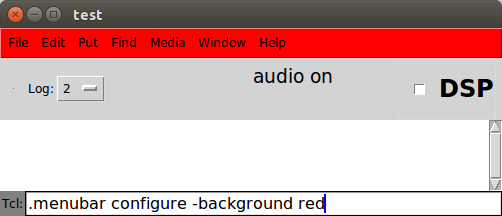
\includegraphics[scale=\Mysize]{tcl_prompt}
	\caption{Prompt tcl como \external}
\end{figure}

\begin{figure}[ht!]
	\centering
	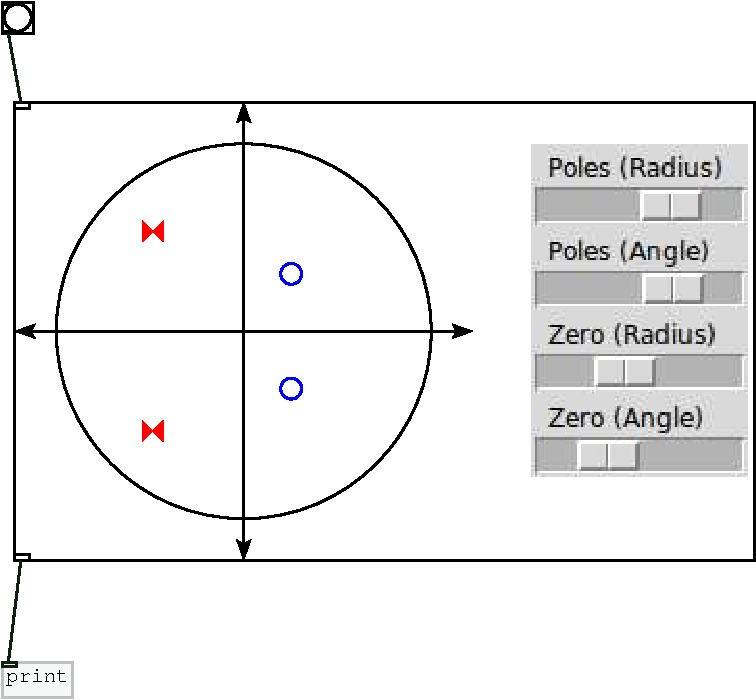
\includegraphics[scale=\Mysize]{filter_circle}
	\caption{Exemplo de \external com GUI TCL}
\end{figure}



